\section{From Flood to Aquifer: Metered Recharge}
\label{sec:recharge}

The water that floods an Indian city in July is water the same region is short of in April. Managed
aquifer recharge is the idea of deliberately putting storm water underground instead of letting it
run off, and it is well studied \cite{mar2026, pavelic2015utfi}. What is usually missing is a
measurement. Most recharge plans assume an infiltration rate and multiply.

We can do better, because we have a physical model that already meters infiltration against a finite
soil capacity, as described in Section~\ref{sec:system}. So we can build recharge structures into the
model, re-simulate the storm, and read off how much water actually went underground rather than
assuming it.

\subsection{Tier A, a state-wide screen}
Choosing where to even build a twin is itself a decision, and doing it by intuition would undo the
point. We screen an entire state first. For each of Karnataka's 27 district units we combine four
free datasets. Central Ground Water Board stage-of-extraction gives the annual ratio of water taken
out to water going in, so above 100\,\% means the aquifer is being mined. A GRACE-assimilated
storage trend gives the direction of change. HydroSHEDS flow accumulation says where runoff
concentrates, because recharge needs water to arrive. SoilGrids conductivity and WorldCover
pervious fraction say whether the ground can take it. The four terms are weighted 0.45 for need,
0.25 for water, 0.15 for soil and 0.15 for land.

The screen ranks Bangalore Rural first at 111\,\% extraction, then Chitradurga at 144\,\%,
Chamarajanagara at 96\,\%, Kolar at 180\,\% and Bangalore Urban at 187\,\%. All are officially
over-exploited or critical.

Two honesty notes travel with this screen. The storage trend input turns out to be effectively
constant across the state, so it contributes nothing to the ranking, and we say so in the artifact
rather than stretching a flat input into apparent signal. And a screen is not a siting. It can say
that a district is depleted \emph{and} has concentrated runoff \emph{and} has pervious ground. It
cannot say build here. Only a re-simulated twin earns a claim in cubic metres.

\subsection{Tier B, twins for six towns, and the measurement}
We then built full 60\,m twins for six Karnataka towns and ran the recharge planner in each, along
with the flood-plain and coastal areas already built. The planner places recharge structures on
pervious ground where water collects, sizes each one, re-simulates, and reports the water that
crossed into the soil column.

\begin{table}[!t]
\centering
\caption{Metered recharge at a 100\,mm storm. Recharge is water that entered the soil column in the
re-simulated model, not an assumed rate. The flood cut column is the measured reduction in street
flooding from the same structures. The plateau towns bank an order of magnitude more of their runoff
than the flood plain and the coast do.}
\label{tab:recharge}
\begin{tabular}{lrrrr}
\toprule
area & sites & recharge (m$^3$) & of runoff & flood cut \\
\midrule
\multicolumn{5}{l}{\emph{Karnataka plateau}}\\
Chikkaballapur   & 4\,323 & 607\,172 & \textbf{16.5\,\%} & 62.7\,\% \\
Kolar            & 4\,875 & 667\,548 & \textbf{14.1\,\%} & 46.9\,\% \\
Doddaballapura   & 4\,122 & 503\,986 & \textbf{10.0\,\%} & 85.4\,\% \\
Chamarajanagara  & 5\,215 & 418\,956 & \textbf{8.1\,\%}  & 88.2\,\% \\
Chitradurga      & 3\,850 & 320\,138 & \textbf{8.0\,\%}  & 49.2\,\% \\
Ramanagara       & 3\,119 & 322\,204 & \textbf{6.3\,\%}  & 76.8\,\% \\
\midrule
\multicolumn{5}{l}{\emph{Flood plain and coast}}\\
Patna-East       & 3\,159 & 102\,013 & 3.3\,\% & 38.4\,\% \\
Patna-West       & 3\,277 & 139\,793 & 2.6\,\% & 22.4\,\% \\
Bengaluru        &    986 &  74\,196 & 1.6\,\% & 4.3\,\% \\
Mumbai-North     & 3\,654 & 114\,711 & 1.1\,\% & 6.2\,\% \\
Patna            & 1\,188 &  32\,714 & 0.7\,\% & 9.1\,\% \\
Mumbai-East      & 2\,693 &  21\,171 & 0.2\,\% & 14.4\,\% \\
Mumbai-West      & 1\,573 &  16\,117 & 0.2\,\% & 7.6\,\% \\
Mumbai-South     &    507 &    $-$534 & 0.0\,\% & 3.7\,\% \\
\bottomrule
\end{tabular}
\end{table}

Table~\ref{tab:recharge} is the result, and the split is the point. The six Karnataka towns send
6.3 to 16.5\,\% of a 100\,mm storm's runoff into the aquifer. The flood plain and the coast manage
0.7 to 3.3\,\%, and Mumbai-South is indistinguishable from zero. That gap is exactly what the
screen predicted and it has a physical reason. On a flood plain the water table is already close to
the surface and the soil column is nearly full, so there is nowhere to put the water. On the
Karnataka plateau the aquifer is mined, hard rock sits under thin soil, and the storage the water
is being invited into is real and empty.

The same structures also cut flooding, by 46.9 to 88.2\,\% in those towns, so this is not a trade
between flood control and water supply. In the places where recharge works, it is the same
intervention.

Fig.~\ref{fig:kolar} shows Kolar, the second-ranked town, with its flood field and the planned
network. Phasing it is costed the same way as storage. Kolar reaches a 10\,\% flood cut with
3\,296 structures holding 6.94 million\,m$^3$, at an indicative \rupee2\,500 per m$^3$ and about
\rupee1\,735 crore.

\begin{figure}[!t]
\centering
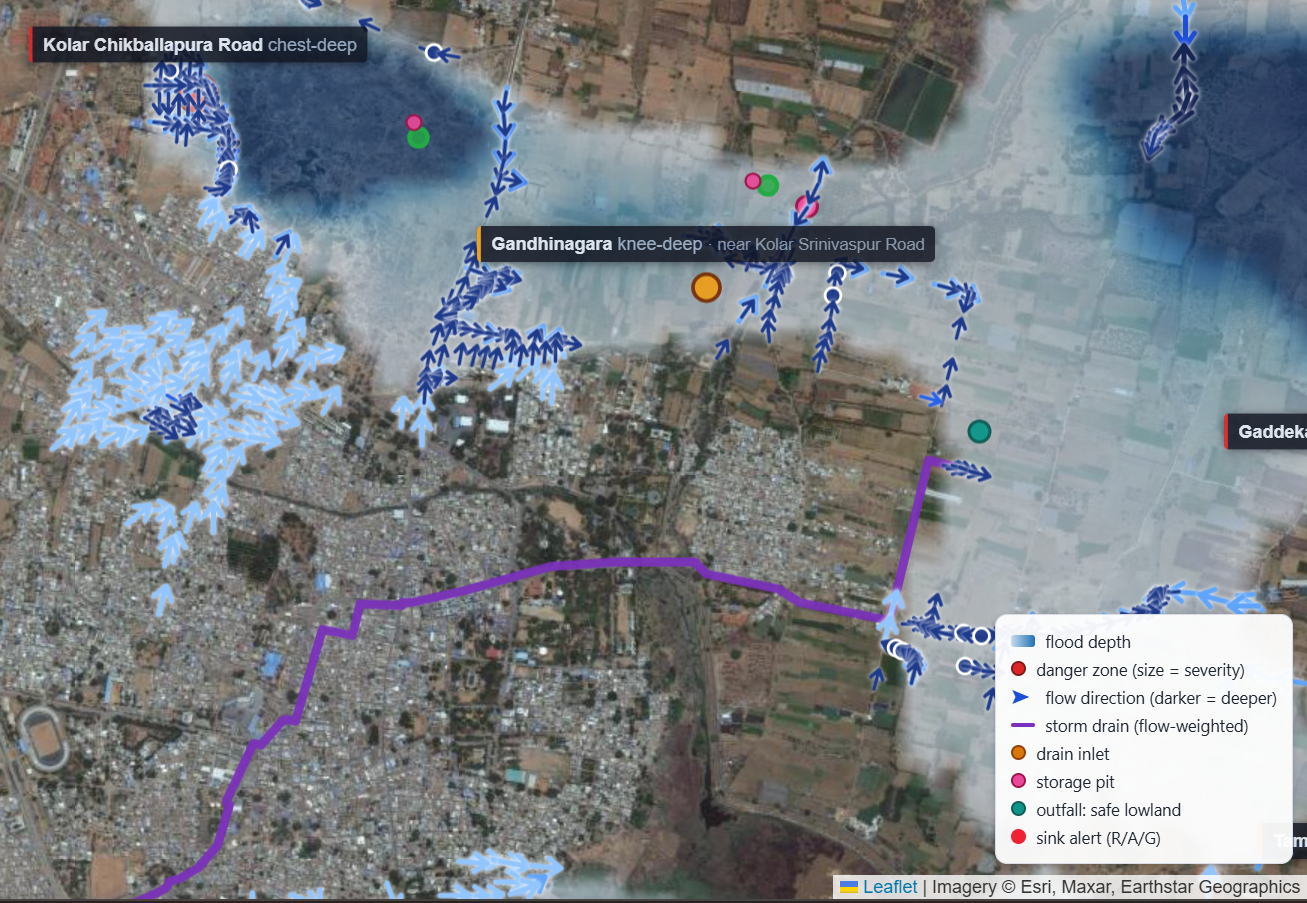
\includegraphics[width=0.99\linewidth]{figures/live_kolar.png}
\caption{Kolar, one of the six Karnataka towns, at a design storm. Kolar district runs at 180\,\%
groundwater extraction, meaning it takes out nearly twice what goes in each year. Blue is predicted
water, arrows are flow, the purple line is the planned trunk to a safe outfall in green, and the
pink circles are storage. Water that currently floods Kolar Chikballapura Road is water the aquifer
under it needs.}
\label{fig:kolar}
\end{figure}

\subsection{What this result does not license}
Two caveats sit on top of these numbers and both are load-bearing.

The recharge \emph{volumes} come from the twin's metered infiltration and depend only on the
physics and the terrain. The site \emph{rankings} additionally use local groundwater level data,
and the well files currently shipped are sample placeholders rather than real measurements, with
the nearest genuine station far outside the area. So the volumes stand and the within-town ordering
of sites should be treated as provisional until Central Ground Water Board station records are
attached. We ship that distinction in the artifact instead of hiding it.

Recharge also has a water quality dimension that a flood model cannot see. Putting urban runoff
underground puts whatever is in that runoff underground too, including sewage and heavy metals.
Parts of Bihar's shallow alluvium carry arsenic, and Karnataka's hard-rock aquifers carry fluoride.
Any real structure needs geotechnical and water-quality screening before construction. This planner
prioritises. It does not certify.
